\section{.NET}
\subsection{Zielsetzungen}
Plattform für vernetzte und integrierte Anwendung - auch mobil, basierend auf Web Services
\begin{itemize}
  \item .NET-Framework
		\begin{itemize}
		\item CLR Common Language Runtime
		\item .NET Framework class library
		\item Compact Framework für Entwicklung von PDA/Mobile -Applikationen
		\item .NET microFramework für Entwicklung von Embedded Systemen
	\end{itemize}
	\item  Visual Studios
	\begin{itemize}
  	\item Unterstützt mehrere .NET-Sprachen: C\#, VB.NET, C++, J\#.NET, F\#, JScript, COBOL, Delphi, \dots	
	\end{itemize}
\end{itemize}

\subsection{Common Language Runtime (CLR)}
\begin{multicols}{2}

	\begin{itemize}
		\item Laufzeitumgebung für .NET Sprachen
			\begin{itemize}
				\item Exceptions
				\item gemeinsames Typensystem (\textbf{C}ommon \textbf{T}ype \textbf{S}ystem)
				\item Thread-Verwaltung
				\item Speicherverwaltung mit Garbage Collection
				\item Just-In-Time Compiler (JIT-Compiler)
				\item Code Access Security
				\item Sprachübergreifenes Debugging
				\item COM-Interoperabilität
				\item Basisklassen mit System-Funktionen
			\end{itemize}
	\end{itemize}
	
	\columnbreak
	
	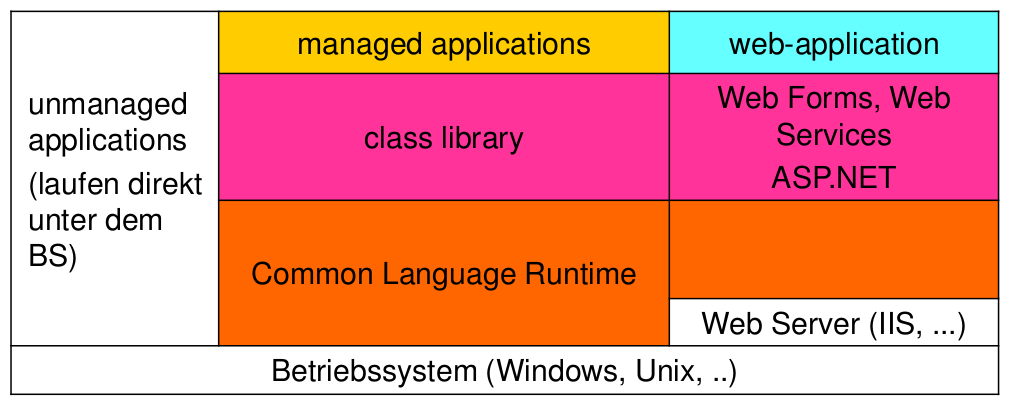
\includegraphics[width=9cm]{images/CSharp/aufbau_dotNet}
	
\end{multicols}
\begin{itemize}
	\item Common Type System (CTS): Gemeinsame Typen für alle Sprachen
		\label{csharpCTS}
		\begin{itemize}
			\item Typen wandern von der Programmiersprache ins Laufzeitsystem
			\item 2 Kategorien von Typen: Reference- und value-Types
			\item Single-rooted $\rightarrow$ Alle Typen sind von System.Object abgeleitet, Value-Types via Boxing
			\item Reflection immer vorhanden, jeder Typ kann zur Laufzeit eingesehen werden.
				Reflection Informationen können über ''custom attributes`` erweitert werden
		\end{itemize}
\end{itemize}


\subsection{MS Intermediate Language (MSIL)}
.NET-Compiler erzeugen keinen ''native`` Code, sondern eine
Prozessor-unabhängige Zwischensprache (MSIL) angereichert mit
Meta-Daten zu den Typen.

IL-Code wird während der Ausführung immer (!) durch einen JIT-Compiler
in echten Maschinencode übersetzt

\begin{itemize}
	\item Zwischencode für virtuelle Stack-Maschine ohne Register
	\item Elemente des CTS (siehe \ref{csharpCTS}) sind fester Bestandteil
	\item Konzepte wie Vererbung und Polymorphie werden unterstützt
	\item Konzipiert für JIT-Compilation, nicht Interpretation (Performance-Vorteile)
	\item Vorteile
		\begin{itemize}
			\item Potential für Portabilität (andere Prozessoren und Betriebssysteme)
			\item Sprache spielt keine Rolle
			\item Type Safety: Beim Laden des Codes können Typen-Sicherheits und andere Checks durchgeführt werden
		\end{itemize}
	\item Nachteile
		\begin{itemize}
			\item Laufzeiteffizienz? Wird wettgemacht durch JIT-Compiler, welcher zur Laufzeit auf den Prozessortyp optimiert
		\end{itemize}

\end{itemize}

\subsection{Metadata}
\begin{itemize}
	\item Kompilation von .NET Sprachen erzeugt ein Modul mit IL-Code \emph{und} Metadaten
	\item Beschreibt Class-, Methods-, Type-definitions
	\item Zugriff über definierte Schnittstellen (Reflection) \newline
	      (Reflections erlauben den Zugriff auf die Metadaten)
	\item Anwendungen
		\begin{itemize}
			\item CLR: Verifikation (Type-Safety) und Memory Management
			\item IDE (z.B. VS IntelliSense)
			\item dynamic binding, erweiterbare Programmsysteme
			\item Analyse eines Modules/Assemblies (z.B ILDASM)
		\end{itemize}
\end{itemize}

\subsection{Assemblies}
Compiler erzeugen Module und Assemblies
\paragraph{Assembly}
\begin{itemize}
	\item exe oder dll file im \textbf{P}ortable \textbf{E}xecutable Format
	\item Auslieferungs- und Ausführungseinheit, dynamisch ladbar
	\item Selbstbeschreibend
	\item Definiert Typ-Scope
	\item Kleinste versionierbare Einheit
	\item Einheit für Security-Überprüfung
\end{itemize}
\paragraph{Aufbau eines Singlefile-Assembly}
\begin{itemize}
	\item Manifest und ein Modul mit Metadata und IL-Code. (Manifest = Assembly Metadaten)
	\item Manifest beschreibt Name, Version, Schnittstelle und Abhängigkeiten zu anderen Assemblies, Sicherheitsattribute, Liste der Typen, \dots
	\item Hat einen Einstiegspunkt (Main, WinMain oder DllMain)
	\item Private Assembly
		\begin{itemize}
			\item Werden nur von einer Applikation benutzt
			\item Direkt im Applikations-Ordner
		\end{itemize}
	\item Shared Assembly
		\begin{itemize}
			\item Von mehreren Applikationen genutzt
			\item eindeutiger Name (Key)
			\item Werdem im Global Assembly Cache (GAC) abgelegt (Tool gacutil.exe)
			\item Version im Manifest
			\item Mehrere Versionen können parallel existieren, jede Applikation verwendet spezifische Version
		\end{itemize}
\end{itemize}

\subsection{Memory Managment}
\begin{itemize}
	\item Garbage Collection
		\begin{itemize}
			\item Automatische Freigabe von nicht mehr verwendetem Objekt-Speicher im Managed-Heap
			\item Kann Heap automatisch umräumen
			\item Programmierer muss sich nicht um Freigabe von Speicher kümmern
			\item Achtung! Komplizierter wenn nicht vom CLR verwaltete Ressourcen verwendet werden.
			\item Weniger Programmabstürze wegen Speicherproblemen
		\end{itemize}
\end{itemize}

\subsection{.NET Framework Class Library}
Umfangreiche Klassenbibliothek
\begin{itemize}
	\item Gemeinsam für alle .NET Sprachen
	\item Bestandteil von .NET als shared Assemblies
	\item Verwendung nur für managed code
	\item Namespaces
	\begin{itemize}
  	\item Sind in hirarchischem Namespace verwaltet	
  	\item Typname muss eindeutig sein innerhalb eines Namespaces
  	\item default Namespace: falls kein expliziter Namespace angegeben ist,
  	      gehört die Typ-Definition zum "Default-Namespace"
	\end{itemize}
\end{itemize}

\subsection{Web Applikations-Plattform ASP.NET}
\begin{itemize}
	\item Web Forms
	\item Web Services
\end{itemize}

\newpage
